% R12. Requires graphicx in the eventual manuscript; not compiled here.
\begin{figure}[ht]
\centering
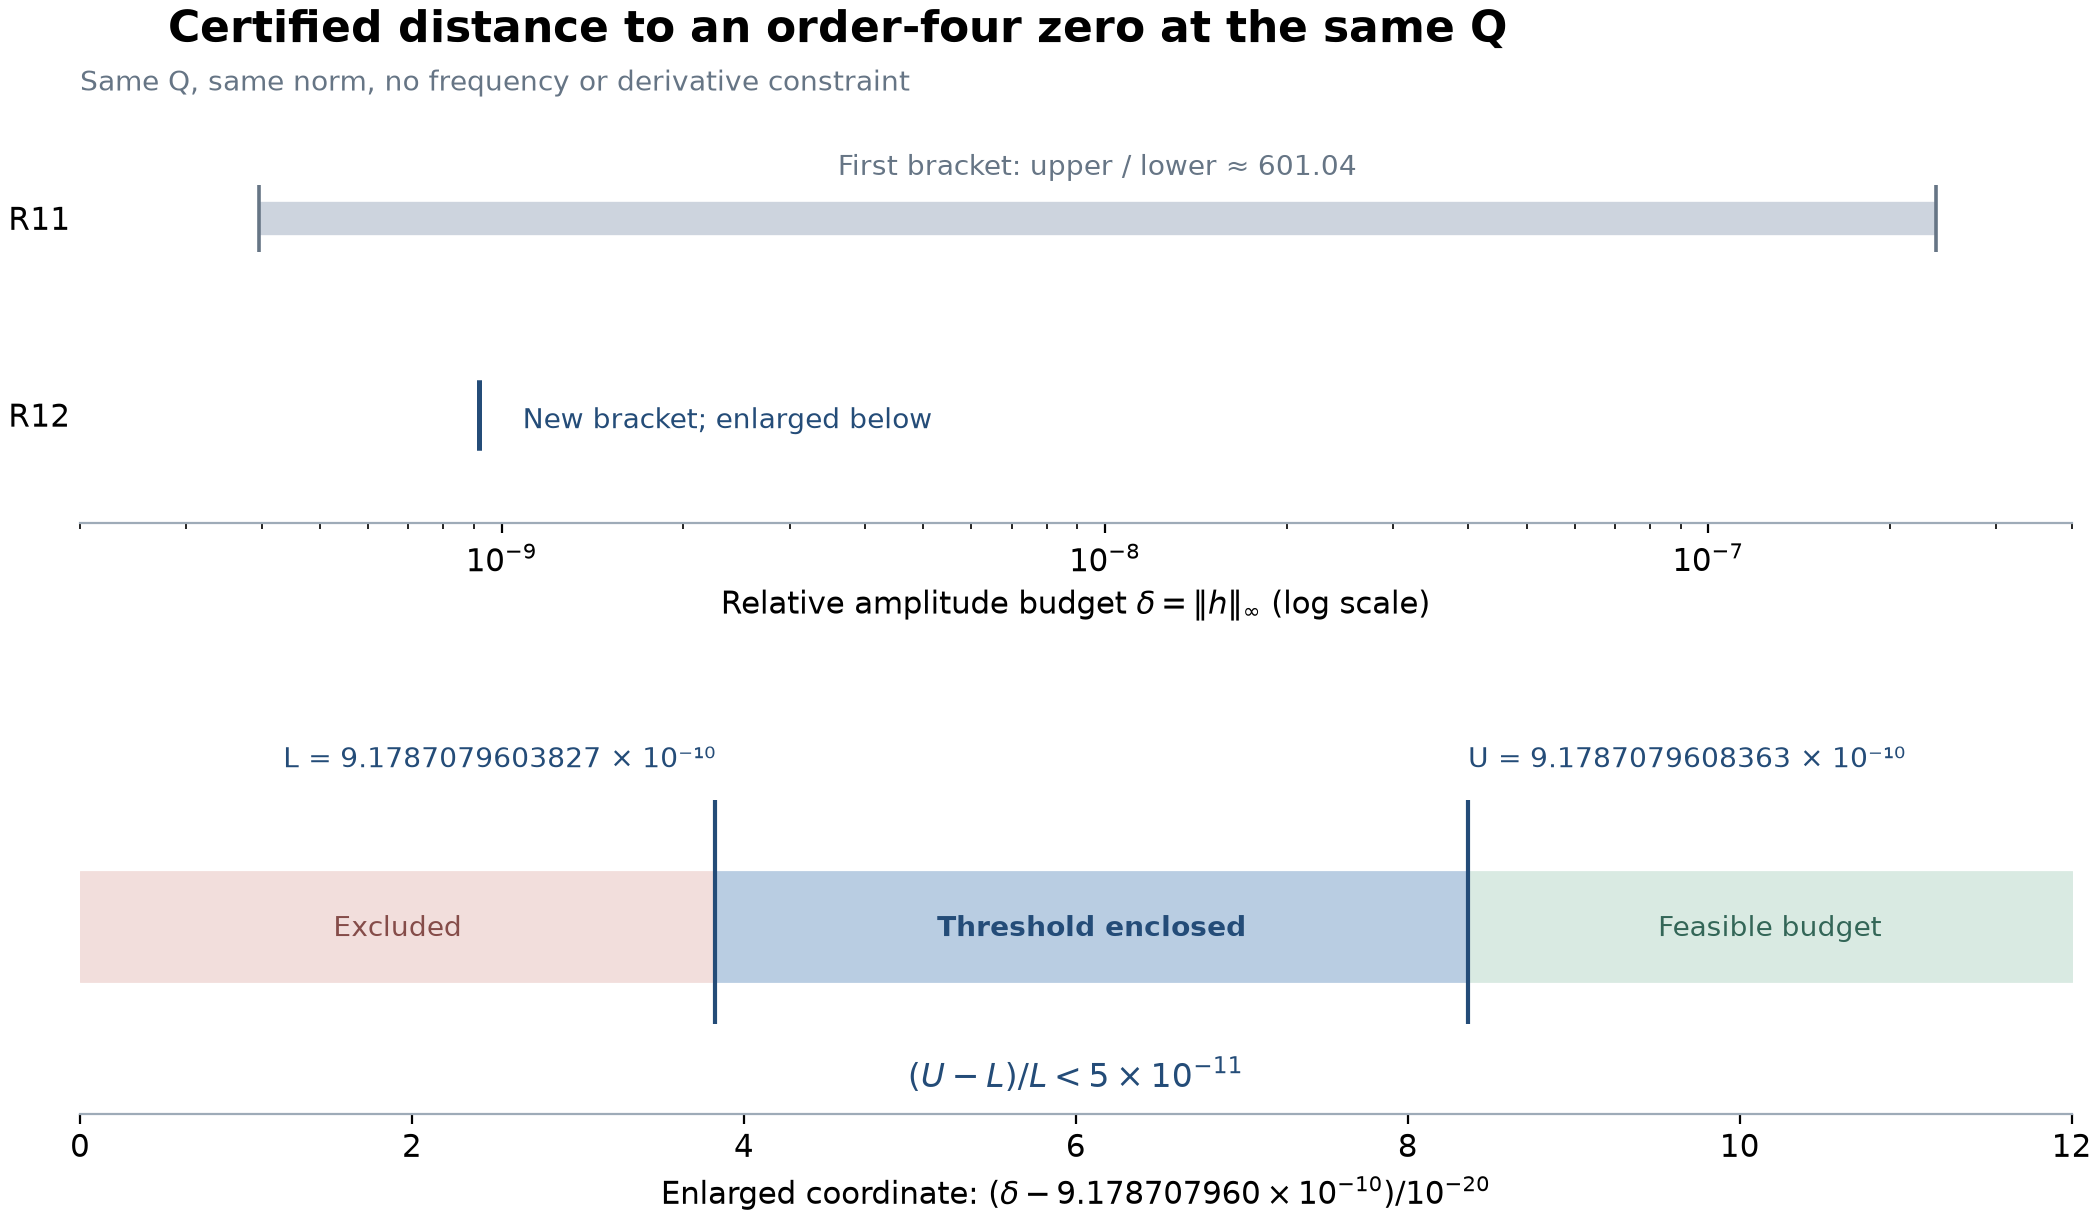
\includegraphics[width=\linewidth]{figures/threshold_contraction.png}
\caption{Certified brackets on the least relative kernel amplitude
needed to turn the original theta example's order-three zero at the
exact point $Q$ into an order-four zero at the same point. The norm
is $\|h\|_\infty$, with no frequency or derivative constraint.
The upper panel compares the first bracket (R11) and the new bracket
(R12) on a logarithmic scale. The latter is too narrow to resolve at
that scale and is enlarged below using the displayed affine coordinate.
The lower bound excludes every admissible multiplier with smaller
norm; the upper bound contains an explicit smooth positive
nondegenerate design. The relative gap of the displayed endpoints
is below $5\times10^{-11}$. No point is labelled as an exactly
computed optimum.}
\label{fig:r12-threshold}
\end{figure}

\begin{figure}[ht]
\centering
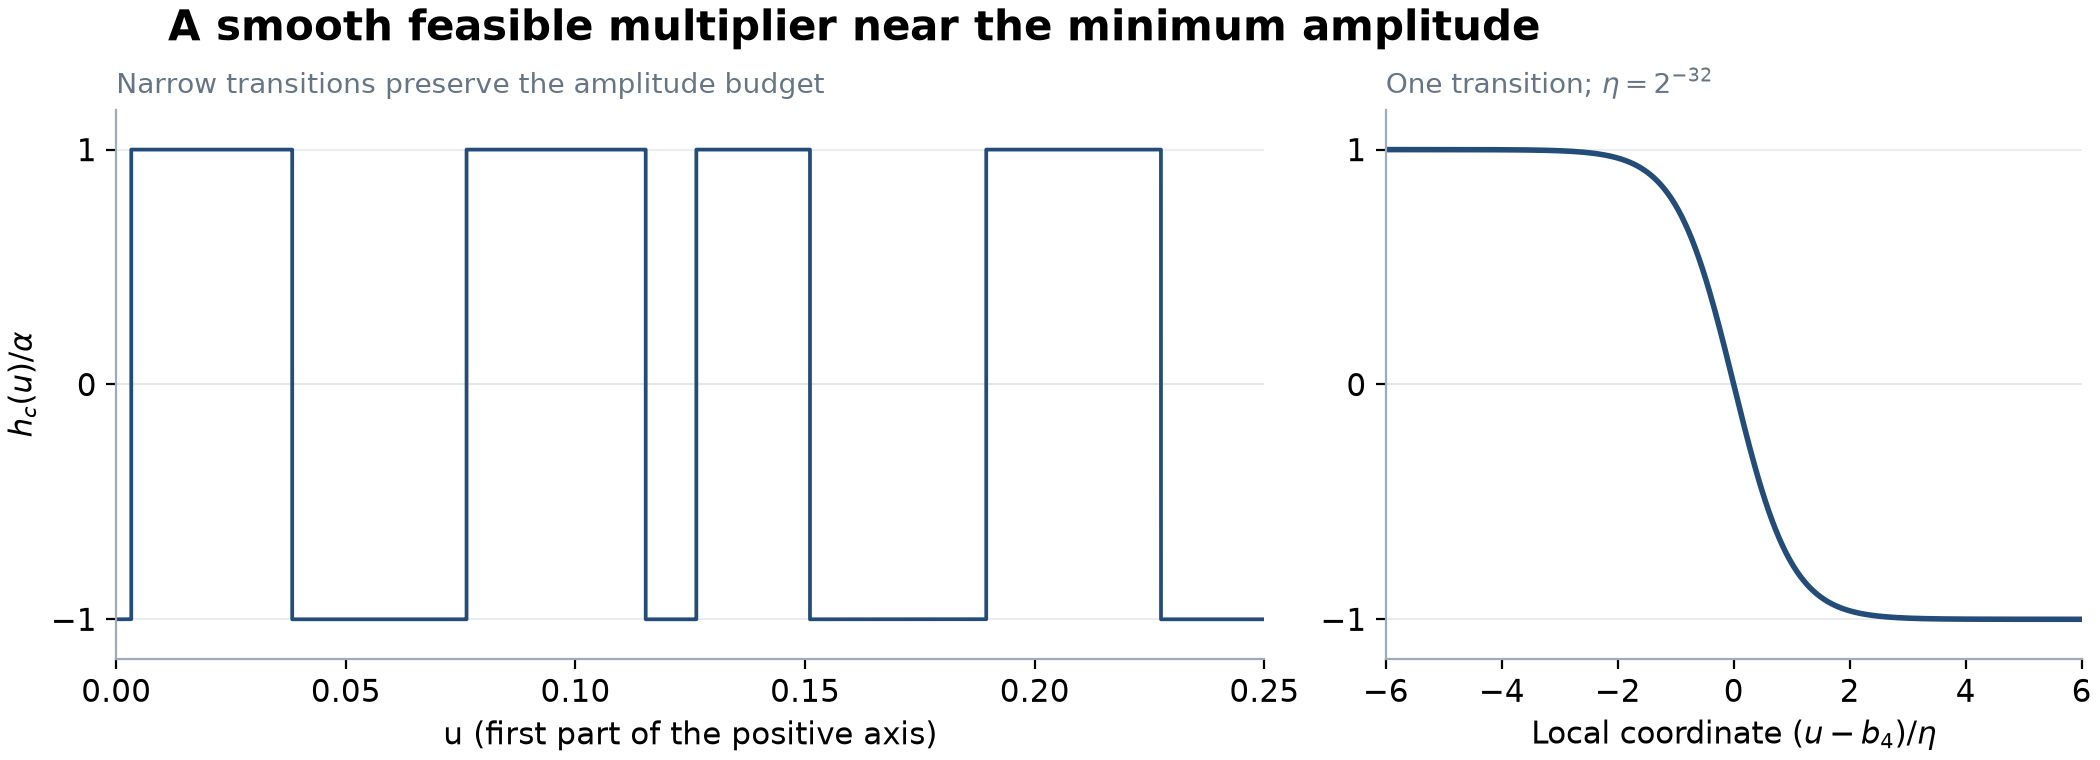
\includegraphics[width=\linewidth]{figures/smooth_near_minimum_design.png}
\caption{Representative rendering of the explicit feasible multiplier
$h_c/\alpha$. The first panel displays $0\le u\le0.25$; the full
template has 28 positive transition knots below $u=1$ and an even
extension. The second panel enlarges the fourth transition in units
of $\eta=2^{-32}$. The curve is real analytic although the transitions
are unresolved on the first panel's scale. Correction coefficients
are drawn at enclosure midpoints; the exact coefficients are defined
by the certified moment system. Exact pinning and norm bounds come
from the certificates, not from these samples. Small amplitude does
not imply a small derivative norm.}
\label{fig:r12-smooth-design}
\end{figure}
